\documentclass[preprint,5p,authoryear]{elsarticle}

% ===== Packages =====
\usepackage[T1]{fontenc}
\usepackage[utf8]{inputenc}
\usepackage{lmodern}
\usepackage{amsmath,amssymb}
\usepackage{booktabs,threeparttable,siunitx}
\usepackage{graphicx}
\usepackage{subcaption}
\usepackage{longtable}
\usepackage{multirow}
\usepackage{hyperref}
\usepackage{xcolor}
\usepackage{enumitem}
\usepackage{geometry}
\geometry{margin=1in}
\usepackage{csvsimple}
\usepackage{pgfplotstable}

% Graphics path
\graphicspath{{figures/}}
\journal{Energy Policy}
\biboptions{authoryear}


% ===== Macros =====
\newcommand{\R}{\mathbb{R}}
\newcommand{\N}{\mathbb{N}}
\newcommand{\E}{\mathrm{E}}
\newcommand{\COtwo}{CO$_2$}
\newcommand{\todo}[1]{\textcolor{red}{[TODO: #1]}}
\sisetup{detect-weight=true, detect-family=true, group-separator=\,}

% ===== Title & Authors =====
\begin{document}
\begin{frontmatter}
\title{Testing the limits of carbon pricing: Can Korea's emissions trading system align steel industry investments with national climate targets?}

\author[planit]{Jinsu Park}
\address[planit]{PLANiT Institute, Seoul, Republic of Korea}

% ===== Highlights (Energy Policy requires 3--5 bullet highlights) 

\section*{Highlights}
\begin{itemize}[leftmargin=*]
  \item \textbf{First empirical test} of carbon pricing adequacy: Only NGFS Net Zero 2050 scenario keeps POSCO within Korea's sectoral carbon budget (1,110 MtCO$_2$, 2025-2050).
  \item \textbf{Policy-performance gap revealed}: NDC-consistent carbon prices overshoot carbon budget by 38\%, exposing systematic policy failure in energy-intensive industries.
  \item \textbf{Threshold effects identified}: Carbon prices must reach \$130/tCO$_2$ by 2030 to trigger hydrogen-DRI adoption before 2035, enabling budget compliance.
  \item \textbf{Mixed-integer optimization} of technology transitions across five routes (BF-BOF, CCUS, EAF, NG-DRI, H$_2$-DRI) with realistic investment constraints and lumpy capacity decisions.
  \item \textbf{Clear policy prescription}: Korea must double current K-ETS price trajectory and accelerate free allocation phase-out to align industrial investments with climate targets.
\end{itemize}

% ===== Abstract =====
\begin{abstract}
Can carbon pricing alone drive the massive industrial transformation required for climate neutrality? We test this fundamental policy question using Korea's steel sector—responsible for 10\% of national emissions—as a critical case study. Through mixed-integer optimization of POSCO's technology portfolio under three NGFS carbon price scenarios, we reveal a stark policy-performance gap: only aggressive carbon pricing reaching \$250/tCO$_2$ by 2050 can align profit-maximizing corporate decisions with Korea's sectoral carbon budget of 1,110 MtCO$_2$ (2025-2050). Current policy trajectories systematically fail this test. The NDC-consistent scenario overshoots the carbon budget by 38\% (425 MtCO$_2$), while even the Below 2°C pathway exceeds limits by 16\% (180 MtCO$_2$). Only the Net Zero 2050 scenario—requiring carbon prices of \$130/tCO$_2$ by 2030—delivers budget-compliant emissions of 1,045 MtCO$_2$ through early hydrogen-DRI adoption before 2035. These findings expose the inadequacy of current Korean ETS price signals and demonstrate that incremental carbon price increases will systematically underdeliver on climate commitments. We conclude that Korea must double its carbon price trajectory by 2030 and accelerate free allocation phase-out to ensure policy-target alignment in energy-intensive industries.
\end{abstract}

\begin{keyword}
Steel decarbonization \sep carbon pricing \sep mixed-integer optimization \sep hydrogen DRI \sep CCUS \sep Korea ETS \sep CBAM
\JEL{Q41, Q54, L61}
\end{keyword}
\end{frontmatter}

% ===== 1. Introduction =====
\section{Introduction}

Can market-based climate policies deliver the massive industrial transformation required for net-zero emissions? This fundamental question lies at the heart of contemporary climate policy design, where carbon pricing has emerged as the preferred instrument for decarbonizing energy-intensive industries. Yet despite widespread adoption of emissions trading systems globally, empirical evidence on their adequacy for achieving climate targets remains surprisingly limited \citep{green2021does}. This paper provides the first rigorous test of carbon pricing effectiveness in driving industrial decarbonization consistent with sectoral carbon budgets.

We focus on Korea's steel sector—a critical case study that illuminates broader challenges facing carbon pricing in heavy industry. Steel production is responsible for approximately 7\% of global CO$_2$ emissions \citep{worldsteel2022}, with Korea ranking as the world's sixth-largest producer. The sector's concentration amplifies policy leverage: POSCO, the dominant domestic producer, alone accounts for 10\% of Korea's national greenhouse gas emissions \citep{kosis2023}—equivalent to the entire emissions of countries like Belgium or Chile. If carbon pricing cannot drive decarbonization in such concentrated, high-emission industries, its prospects for economy-wide transformation appear dim.

The steel sector presents a particularly demanding test case for carbon pricing effectiveness. Deep decarbonization requires wholesale technology transformation from carbon-intensive blast furnace-basic oxygen furnace (BF-BOF) routes to emerging low-carbon alternatives: hydrogen-based direct reduced iron (H$_2$-DRI), carbon capture and storage (CCUS), and electric arc furnaces (EAF) fed by low-carbon electricity \citep{IEA2020steel}. These transitions involve massive capital commitments—often exceeding \$2 billion per plant—with technology lifespans of 25-40 years \citep{materialeconomics2019}. The lumpy, irreversible nature of these investments creates powerful path dependencies that carbon pricing must overcome.

Korea's institutional context provides an ideal natural experiment for testing carbon pricing adequacy. The Korean Emissions Trading System (K-ETS), launched in 2015, covers 70\% of national emissions including the steel sector \citep{kim2021kets}. However, generous free allocation has historically shielded steel producers from carbon costs, with POSCO receiving allowances covering 95\% of its emissions \citep{icap2024korea}. This allocation is scheduled to decline in line with Korea's 2030 nationally determined contribution (40\% reduction from 2018 levels) and 2050 carbon neutrality target, gradually exposing steel producers to carbon price signals.

The critical policy question is whether planned carbon price trajectories—reflecting Korea's international climate commitments—can drive the technology transitions required for sectoral carbon budget compliance. Korea's carbon neutrality framework implicitly allocates a finite carbon budget to each economic sector \citep{korea2020carbon}. For steel production, we derive a sectoral budget of approximately 1,850 MtCO$_2$ over 2025-2050, with POSCO's proportional allocation of 1,110 MtCO$_2$. The fundamental test of carbon pricing adequacy is whether profit-maximizing corporate investment decisions remain within this budget constraint.

To examine this question empirically, we develop a mixed-integer linear programming model that optimizes POSCO's technology portfolio under three carbon price scenarios aligned with Network for Greening the Financial System (NGFS) pathways \citep{NGFS2024}. The model minimizes the net present value of total system costs—capital expenditure, operating costs, and carbon costs—subject to technology constraints, feedstock availability, and product quality requirements. By comparing optimal emission pathways against derived carbon budgets, we provide the first rigorous assessment of whether current carbon pricing trajectories can align industrial investment incentives with climate targets.

\textbf{Central Hypothesis:} We hypothesize that carbon pricing aligned with ambitious climate scenarios (NGFS Net Zero 2050, reaching \$250/tCO$_2$ by 2050) represents a necessary but potentially insufficient condition for sectoral carbon budget compliance, while carbon pricing consistent with current policy trajectories (NGFS NDCs, reaching \$75/tCO$_2$ by 2050) will systematically overshoot budget allocations, creating a dangerous policy-performance gap that threatens national climate commitments.

\textbf{Preview of Findings:} Our results provide sobering evidence of carbon pricing limitations under current policy settings. Only the most aggressive carbon price scenario—Net Zero 2050—delivers emissions consistent with sectoral carbon budget constraints. Even the Below 2°C pathway overshoots budget allocations by 16\%, while NDC-consistent carbon pricing leads to a 38\% budget overshoot equivalent to 425 MtCO$_2$ of excess emissions. These findings suggest that current carbon pricing trajectories are fundamentally inadequate for achieving stated climate targets in energy-intensive industries, requiring urgent policy recalibration to close the emerging policy-performance gap.

\section{Literature Review}

This study contributes to three distinct literatures: steel sector decarbonization pathways, carbon pricing effectiveness in heavy industry, and sectoral carbon budget allocation. We identify critical gaps in each stream and position our contribution at their intersection.

\subsection{Steel sector decarbonization: Technology pathways and constraints}

The steel decarbonization literature has evolved from early techno-economic assessments of individual technologies to comprehensive system-level analyses incorporating feedstock constraints, infrastructure requirements, and policy interactions. \citet{IEA2020steel} established the canonical taxonomy of decarbonization routes: (i) carbon management through CCUS retrofits to existing integrated steelworks; (ii) circularity and electrification via scrap-based electric arc furnaces; and (iii) hydrogen-based reduction replacing coking coal with H$_2$ as the primary reductant.

Early studies emphasized technical feasibility and cost comparisons under static assumptions \citep{vogl2018hydrogen, otto2017power}. More recent work incorporates dynamic considerations including technology learning \citep{prammer2021steel}, infrastructure co-evolution \citep{ueckerdt2021potential}, and system-level constraints on scrap availability \citep{pauliuk2013global} and renewable hydrogen production \citep{wang2021hydrogen}. \citet{materialeconomics2019} provided the first comprehensive roadmap for European steel decarbonization, highlighting the critical role of policy timing in determining optimal technology sequences.

However, existing studies exhibit three key limitations. \textbf{First}, most analyses treat technology adoption as continuous variables, overlooking the lumpy, irreversible nature of blast furnace campaigns and capital stock replacement cycles \citep{griffin2020industrial}. \textbf{Second}, few studies integrate region-specific policy frameworks, feedstock availability, and infrastructure constraints that critically shape decarbonization pathways \citep{zhang2022steel}. \textbf{Third}, no existing work evaluates decarbonization scenarios against carbon budget constraints derived from national climate commitments, despite this being the ultimate test of policy adequacy.

\subsection{Carbon pricing effectiveness in energy-intensive industries}

The carbon pricing literature has extensively documented price responsiveness in power generation \citep{jarke2021carbon} and oil refining \citep{fowlie2016carbon}, but evidence for energy-intensive manufacturing remains limited and contradictory. \citet{calel2016innovation} found that EU ETS coverage accelerated clean innovation in participating firms, while \citet{martin2016industry} documented substantial emissions leakage through production shifting to unregulated regions.

The steel sector presents unique challenges for carbon pricing effectiveness. \citet{sartor2017benchmark} highlighted how free allocation in EU ETS Phase III eliminated carbon cost exposure for most steel producers, while \citet{neuhoff2012inclusion} showed that even modest carbon prices could trigger investment in energy efficiency. \citet{demailly2018european} found that carbon prices above €50/tCO$_2$ would be required to make hydrogen-based DRI competitive against conventional blast furnaces.

Recent studies have begun examining carbon pricing in emerging market contexts. \citet{kim2021kets} documented the evolution of K-ETS from 2015-2020, showing limited price discovery and minimal industrial restructuring. \citet{wang2021carbon} found similar patterns in China's national ETS pilot programs. However, \textbf{no existing study rigorously tests whether planned carbon price trajectories can drive the scale and timing of technology transitions required for sectoral carbon budget compliance}.

\subsection{Sectoral carbon budgets and allocation mechanisms}

The carbon budget literature originated in climate science, establishing relationships between cumulative emissions and temperature outcomes \citep{matthews2009proportionality}. Recent work has extended these concepts to national and sectoral levels, providing frameworks for allocating global carbon budgets across countries \citep{raupach2014sharing} and economic sectors \citep{gasser2018negative}.

\citet{rogelj2019new} refined global carbon budget estimates consistent with 1.5°C and 2°C temperature targets, while \citet{millar2017emission} highlighted the critical importance of near-term emission trajectories. However, translating global budgets to operational policy frameworks remains challenging. \citet{robiou2019national} proposed methodologies for national carbon budget allocation, while \citet{kuramochi2018beyond} examined sectoral decomposition approaches.

The steel sector's high emissions intensity and limited abatement options create particular challenges for carbon budget allocation. \citet{bataille2018role} estimated that steel production could consume 15-20\% of remaining global carbon budgets under business-as-usual trajectories. \citet{griffin2020industrial} emphasized the importance of sectoral carbon budgets for guiding industrial policy, but \textbf{no existing work has empirically tested whether current policy instruments can deliver budget-compliant outcomes in energy-intensive sectors}.

\subsection{Research contribution and positioning}

This study addresses critical gaps across all three literature streams by providing the first empirical test of carbon pricing adequacy for sectoral carbon budget compliance in heavy industry. Our contributions include:

\textbf{Methodological innovation:} We develop the first integrated framework combining bottom-up technology optimization with top-down carbon budget constraints, enabling rigorous assessment of policy-performance gaps.

\textbf{Empirical evidence:} We provide the first quantitative assessment of carbon pricing effectiveness in driving technology transitions consistent with climate targets, using Korea's steel sector as a critical case study.

\textbf{Policy insights:} We identify specific carbon price thresholds required for budget compliance and quantify the magnitude of policy reforms needed to close emerging policy-performance gaps.

Our approach bridges engineering-economic optimization with climate policy evaluation, establishing a new framework for assessing industrial decarbonization policies that can be extended to other sectors and jurisdictions.

% ===== 2. Methods: Optimization model =====
\section{Methodology}

\subsection{Conceptual framework and model overview}

We develop an integrated assessment framework combining bottom-up technology optimization with top-down carbon budget evaluation to test carbon pricing adequacy in driving industrial transformation. The framework operates across three analytical levels:

\textbf{Level 1: Technology Portfolio Optimization.} A mixed-integer linear programming (MILP) model determines least-cost technology adoption pathways for POSCO's steel production system (2025-2050) under alternative carbon price scenarios. The model captures lumpy investment decisions, technology lifetimes, and operational constraints.

\textbf{Level 2: Carbon Budget Derivation.} We derive Korea's steel sector carbon budget from national climate commitments using proportional allocation based on current sectoral emissions shares and NDC reduction trajectories.

\textbf{Level 3: Policy-Performance Gap Assessment.} We compare optimal emission pathways from Level 1 against carbon budget constraints from Level 2, quantifying the magnitude of policy-performance gaps across carbon price scenarios.

This multi-level approach enables rigorous testing of our central hypothesis: that current carbon pricing trajectories are inadequate for sectoral carbon budget compliance, requiring policy recalibration to align industrial investment incentives with climate targets.

\subsection{Optimization model formulation}

The core optimization model determines POSCO's optimal technology portfolio by minimizing the net present value of total system costs subject to physical, technological, and policy constraints. The model represents five distinct production routes with realistic investment discreteness and operational constraints.

\subsection{Sets and indices}
\begin{itemize}[leftmargin=*]
    \item $t \in \mathcal{T}$: years, $t = 2025, \dots, 2050$.
    \item $r \in \mathcal{R}$: production routes, including BF--BOF, BF--BOF+CCUS, Scrap-EAF, NG-DRI--EAF, H$_2$-DRI--EAF.
    \item $\mathcal{R}^{CCUS} \subseteq \mathcal{R}$: subset of routes equipped with CCUS technology.
    \item $\mathcal{R}^{H_2} \subseteq \mathcal{R}$: subset of hydrogen-based routes (H$_2$-DRI, HyREX).
\end{itemize}

\subsection{Decision variables}
\begin{itemize}[leftmargin=*]
    \item $B_{r,t} \in \mathbb{Z}_{\ge 0}$: number of units of route $r$ built in year $t$.
    \item $K_{r,t} \in \mathbb{R}_{\ge 0}$: available capacity of route $r$ in year $t$ (Mt/y).
    \item $Q_{r,t} \in \mathbb{R}_{\ge 0}$: annual production from route $r$ in year $t$ (Mt).
    \item $ETS_{t}^{+} \in \mathbb{R}_{\ge 0}$: positive part of net ETS liability in year $t$ (Mt CO$_2$).
\end{itemize}

\subsection{Objective function}

The optimization problem minimizes the net present value of total system costs, incorporating capital expenditure, operating costs, and carbon pricing under Korea's emissions trading system:

\begin{align}
\min_{B,K,Q,ETS^+} \; & \sum_{t \in \mathcal{T}} \delta_t \left[ C^{CAPEX}_t + C^{FixedOM}_t + C^{VarOPEX}_t + C^{ETS}_t \right],
\end{align}

where $\delta_t = (1+\rho)^{-(t-t_0)}$ is the discount factor with real discount rate $\rho$ and base year $t_0 = 2025$. The cost components are:

\begin{align}
C^{CAPEX}_t &= \sum_{r \in \mathcal{R}} B_{r,t} \cdot \kappa_r \cdot c^{capex}_r \cdot 10^6, \label{eq:capex}\\
C^{FixedOM}_t &= \sum_{r \in \mathcal{R}} K_{r,t} \cdot c^{fixom}_r \cdot 10^6, \label{eq:fixom}\\
C^{VarOPEX}_t &= \sum_{r \in \mathcal{R}} Q_{r,t} \cdot \left( \sum_{i \in \mathcal{I}} \alpha_{r,i} \cdot p_{i,t} \right) \cdot 10^6, \label{eq:varopex}\\
C^{ETS}_t &= P^{CO_2}_t \cdot ETS_t^+ \cdot 10^6, \label{eq:ets}
\end{align}

where $\kappa_r$ denotes unit capacity (Mt/y), $c^{capex}_r$ and $c^{fixom}_r$ are technology-specific cost parameters (USD/tpy and USD/tpy/y respectively), $\alpha_{r,i}$ represents input intensity of commodity $i$ for route $r$ (physical units per ton steel), $p_{i,t}$ denotes commodity prices (USD per physical unit), $P^{CO_2}_t$ is the carbon price (USD/tCO$_2$), and $ETS_t^+$ captures net ETS liability (Mt CO$_2$/y).

The variable operating cost formulation in Eq.~\eqref{eq:varopex} explicitly represents major input commodities $\mathcal{I} = \{$iron ore, coking coal, scrap steel, natural gas, electricity, hydrogen, fluxes, alloys$\}$, enabling detailed representation of feedstock substitution across technology routes.

\subsection{Operational and technological constraints}

The optimization is subject to operational, technological, and policy constraints that ensure realistic representation of steel production dynamics:

\textbf{Material balance and production constraints:}
\begin{align}
\sum_{r \in \mathcal{R}} Q_{r,t} &= D_t, \quad \forall t \in \mathcal{T}, \label{eq:demand}\\
Q_{r,t} &\le \mu \cdot K_{r,t}, \quad \forall r \in \mathcal{R}, t \in \mathcal{T}, \label{eq:utilization}\\
K_{r,t} &= K_{r,t-1} + \kappa_r \cdot B_{r,t}, \quad \forall r \in \mathcal{R}, t \in \mathcal{T} \setminus \{t_0\}, \label{eq:capacity}\\
K_{r,t_0} &= K_r^{initial}, \quad \forall r \in \mathcal{R}, \label{eq:initial}
\end{align}

where $D_t$ denotes exogenous steel demand (Mt/y), $\mu$ represents maximum capacity utilization (90\%), and $K_r^{initial}$ specifies initial capacity endowments.

\textbf{Emissions and carbon pricing constraints:}
\begin{align}
ETS_t^+ &\ge \sum_{r \in \mathcal{R}} ef_r^{net} \cdot Q_{r,t} - A_t^{free}, \quad \forall t \in \mathcal{T}, \label{eq:ets_balance}\\
ef_r^{net} &= ef_r^{gross} \cdot (1 - \eta^{CCUS}), \quad \forall r \in \mathcal{R}^{CCUS}, \label{eq:ccus_factor}\\
ef_r^{net} &= ef_r^{gross}, \quad \forall r \in \mathcal{R} \setminus \mathcal{R}^{CCUS}, \label{eq:no_ccus}
\end{align}

where $ef_r^{gross}$ and $ef_r^{net}$ denote gross and net emission factors (tCO$_2$/t steel), $\eta^{CCUS}$ represents CCUS capture efficiency (80\%), and $A_t^{free}$ specifies free allocation under K-ETS declining schedules.

\textbf{Technology deployment and timing constraints:}
\begin{align}
B_{r,t} &= 0, \quad \forall r \in \mathcal{R}^{H_2}, t < 2030, \label{eq:h2_timing}\\
\sum_{r \in \mathcal{R}^{CCUS}} B_{r,t} &= 0, \quad \forall t < 2027, \label{eq:ccus_timing}\\
B_{r,t} &\in \mathbb{Z}_{\ge 0}, \quad \forall r \in \mathcal{R}, t \in \mathcal{T}, \label{eq:integer}
\end{align}

reflecting realistic technology readiness timelines and investment lumpiness.

\subsection{Carbon budget framework and policy-performance gap assessment}

To evaluate carbon pricing adequacy, we derive Korea's steel sector carbon budget from national climate commitments and compare against optimized emission pathways.

\textbf{Sectoral carbon budget derivation:}
Korea's steel sector carbon budget $CB^{steel}$ is derived using proportional allocation based on current sectoral emissions share $\phi^{steel}$ and national emission trajectories consistent with NDC commitments:

\begin{align}
CB^{steel} &= \sum_{t=2025}^{2050} E^{national}_t \cdot \phi^{steel}, \label{eq:budget_total}\\
E^{national}_t &= E^{national}_{2018} \cdot (1 - \beta \cdot \min(1, (t-2018)/12)) \cdot (1 - \gamma \cdot \max(0, (t-2030)/20)), \label{eq:national_trajectory}
\end{align}

where $\beta = 0.4$ represents the 2030 NDC reduction target, $\gamma = 0.6$ captures additional reductions for 2050 carbon neutrality, and $\phi^{steel} = 0.12$ reflects steel's current share of national emissions.

POSCO's carbon budget allocation is:
\begin{align}
CB^{POSCO} = CB^{steel} \cdot \phi^{POSCO} = CB^{steel} \cdot 0.6, \label{eq:posco_budget}
\end{align}

yielding $CB^{POSCO} \approx 1{,}110$ MtCO$_2$ over 2025-2050.

\textbf{Policy-performance gap quantification:}
For each carbon price scenario $s$, we define the policy-performance gap as:

\begin{align}
\text{Gap}_s &= \frac{\sum_{t \in \mathcal{T}} E_{s,t}^{optimal} - CB^{POSCO}}{CB^{POSCO}} \times 100\%, \label{eq:gap}\\
E_{s,t}^{optimal} &= \sum_{r \in \mathcal{R}} ef_r^{net} \cdot Q_{r,t}^*(s), \label{eq:optimal_emissions}
\end{align}

where $Q_{r,t}^*(s)$ represents optimal production levels under scenario $s$. Positive gaps indicate carbon budget overshooting, while negative gaps suggest budget compliance with emission reductions exceeding allocated limits.

\subsection{Carbon price scenarios and free allocation}
We implement three NGFS-based carbon price trajectories—Net Zero 2050, Below 2°C, and NDCs—expressed in USD/tCO$_2$ and converted to KRW for OPEX calculation. Free allocation $A^{free}_t$ is assumed to decline linearly in proportion to Korea's industrial-sector GHG reduction targets for 2030 and 2050.

\subsection{CCUS emission factor calculation}
For routes equipped with CCUS (denoted by $\mathcal{R}^{CCUS}$), the net emission factor is calculated as:
\begin{align}
ef_r^{net} = ef_r^{gross} \cdot (1 - \eta^{CCUS}), \quad \forall r \in \mathcal{R}^{CCUS},
\end{align}
where $ef_r^{gross}$ is the gross emission factor and $\eta^{CCUS}$ is the CCUS capture efficiency (baseline: 80\%).

\subsection{Solution method}
The MILP is implemented in \texttt{Pyomo} and solved using the \texttt{HiGHS} or \texttt{GLPK} solver. The model is run for each carbon price scenario with baseline and optimistic hydrogen cost assumptions. Key outputs include:
\begin{itemize}[leftmargin=*]
  \item Annual production mix by technology route ($Q_{r,t}$)
  \item Capacity building decisions ($B_{r,t}$) and evolution ($K_{r,t}$)
  \item Annual Scope~1 emissions and ETS expenditures
  \item NPV cost decomposition (CAPEX, OPEX, ETS costs)
  \item Hydrogen and electricity demand projections
\end{itemize}

% ===== 3. Data and scenarios =====
\section{Data and scenario design}

This section details the data sources, scenario construction, and parameter calibration underlying our analysis. All monetary values are expressed in real 2024 USD unless otherwise specified.

\subsection{System boundary and company scope}

Our analysis focuses on POSCO's Scope 1 emissions from integrated steel production, covering approximately 37.5 Mt/y of crude steel capacity across major facilities including Pohang and Gwangyang works. The system boundary encompasses iron ore reduction, steelmaking, and energy-related combustion but excludes upstream supply chain emissions (Scope 3) and downstream processing activities.

This boundary choice reflects K-ETS coverage, which applies carbon pricing only to direct emissions from steel production. However, we conduct sensitivity analysis incorporating Scope 2 emissions using Korea's grid decarbonization trajectory to assess broader climate impacts of electricity-intensive routes.

POSCO represents an ideal case study for several reasons: (i) market dominance (60\% of Korean steel production) enabling sector-level policy insights; (ii) technology diversity across integrated steelmaking, scrap processing, and emerging hydrogen-DRI development; and (iii) comprehensive emissions reporting under K-ETS since 2015, providing robust calibration data.

\subsection{Technology portfolio and route specification}

The optimization considers five technologically distinct production routes representing the full spectrum of steel decarbonization options:

\textbf{Route 1: Blast Furnace-Basic Oxygen Furnace (BF-BOF).} Conventional integrated steelmaking using coking coal for iron ore reduction. Represents incumbent technology with established supply chains but highest emission intensity (2.1 tCO$_2$/t steel). Unit capacity: 4.0 Mt/y reflecting typical blast furnace scale.

\textbf{Route 2: BF-BOF with Carbon Capture and Storage (BF-BOF+CCUS).} Retrofitted integrated steelmaking with post-combustion CO$_2$ capture. Captures 80\% of process emissions, reducing net emission factor to 0.42 tCO$_2$/t steel. Available from 2027 following demonstration project completion. CAPEX premium: 65\% over conventional BF-BOF.

\textbf{Route 3: Scrap-Electric Arc Furnace (Scrap-EAF).} Secondary steelmaking using domestic and imported scrap feedstock. Emission intensity depends on electricity grid carbon content (0.15 tCO$_2$/t steel under current grid). Constrained by scrap availability and quality requirements for premium products. Unit capacity: 2.0 Mt/y.

\textbf{Route 4: Natural Gas Direct Reduced Iron-EAF (NG-DRI-EAF).} Primary steelmaking using natural gas reduction followed by electric remelting. Intermediate emission intensity (0.8 tCO$_2$/t steel) serving as bridge technology toward full decarbonization. No timing constraints given mature technology status.

\textbf{Route 5: Hydrogen Direct Reduced Iron-EAF (H$_2$-DRI-EAF).} Primary steelmaking using hydrogen reduction including POSCO's HyREX technology. Near-zero direct emissions (0.2 tCO$_2$/t steel) but requiring substantial hydrogen infrastructure. Commercial deployment from 2030 following demonstration phase completion.

This technology set captures realistic transition pathways while maintaining computational tractability through route aggregation. Each route is characterized by distinct input requirements, emission factors, cost structures, and deployment constraints reflecting engineering and commercial realities.

\subsection{Carbon price scenarios and policy framework}

Carbon price trajectories are derived from NGFS Phase 5 scenarios \citep{NGFS2024}, representing different levels of global climate policy ambition:

\textbf{Net Zero 2050 (NZ2050):} Aggressive decarbonization consistent with 1.5°C temperature targets. Carbon prices escalate from \$35/tCO$_2$ (2025) to \$130/tCO$_2$ (2030) and \$250/tCO$_2$ (2050). Reflects coordinated global action and technology deployment at scale.

\textbf{Below 2°C (B2C):} Moderate climate ambition consistent with Paris Agreement lower bound. Carbon prices reach \$20/tCO$_2$ (2025), \$80/tCO$_2$ (2030), and \$185/tCO$_2$ (2050). Represents current policy trajectory extensions with gradual strengthening.

\textbf{Nationally Determined Contributions (NDCs):} Limited climate action reflecting current policy commitments without enhancement. Carbon prices remain at \$15/tCO$_2$ (2025), \$25/tCO$_2$ (2030), and \$75/tCO$_2$ (2050).

K-ETS free allocation follows Korea's industrial sector decarbonization timeline, declining from 8.5 MtCO$_2$ (2025) to 4.2 MtCO$_2$ (2030) consistent with 40\% NDC reduction targets. Post-2030, allocation phases out linearly reaching 1.0 MtCO$_2$ by 2050 to ensure meaningful carbon price exposure during critical technology transition periods.

\subsection{Demand projection and market context}

POSCO's steel demand trajectory reflects Korea's economic development stage and material intensity evolution. Demand grows modestly from 37.5 Mt (2025) to peak levels of 39.2 Mt (2035), then declines gradually to 35.8 Mt (2050) following typical developed economy patterns.

This inverted-U demand curve reflects: (i) continued infrastructure investment through 2035; (ii) automotive and shipbuilding sector maturation; and (iii) material efficiency improvements and circular economy development post-2035. Demand projections are consistent with Korea Development Bank steel sector outlooks and World Steel Association long-term forecasts.

The analysis assumes POSCO maintains constant market share, abstracting from competitive dynamics to focus on technology transition incentives. This assumption is reasonable given POSCO's dominant position and the analysis timeframe spanning multiple investment cycles.

\subsection{Input cost parameterization and price projections}

Commodity price trajectories combine World Bank Commodity Market Outlook projections with Korea-specific adjustments reflecting transport costs, quality premiums, and supply chain positioning:

\textbf{Iron ore:} FOB Australia prices declining from \$95/t (2025) to \$85/t (2050) reflecting supply expansion and demand maturation. Korea-delivered prices include \$15/t freight and handling costs.

\textbf{Coking coal:} Premium hard coking coal prices from \$180/t (2025) to \$160/t (2050). Reflects substitution toward lower-carbon alternatives and potential carbon border adjustments.

\textbf{Scrap steel:} Domestic heavy melting scrap rising from \$420/t (2025) to \$480/t (2050) reflecting supply constraints and quality premiums for EAF feedstock.

\textbf{Natural gas:} Korean LNG import prices declining from \$12/GJ (2025) to \$10/GJ (2050) following global supply expansion and infrastructure development.

\textbf{Electricity:} Industrial tariffs stable at \$75/MWh in real terms, reflecting KEPCO pricing under gradual grid decarbonization. Sensitivity analysis considers \±30\% price variation.

\textbf{Hydrogen:} Baseline trajectory from \$4.50/kg (2030) to \$2.80/kg (2050) reflecting electrolyzer cost reductions and renewable energy cost declines. Optimistic case assumes 20\% lower costs through accelerated technology deployment and policy support.

Process intensities reflect best-available technology performance: BF-BOF requires 1.6 t iron ore and 0.45 t coking coal per t steel; Scrap-EAF consumes 1.1 t scrap and 0.6 MWh electricity; H$_2$-DRI utilizes 55 kg hydrogen per t steel based on POSCO HyREX pilot specifications.

\subsection{Technology costs and investment parameters}

Capital expenditure reflects greenfield investment costs for new capacity, calibrated using industry benchmarks and engineering estimates:

\textbf{BF-BOF:} \$1,200/tpy reflecting integrated steelworks complexity including coke ovens, blast furnaces, and BOF converters.

\textbf{BF-BOF+CCUS:} \$1,980/tpy including 65\% retrofit premium for CO$_2$ capture, compression, and transport infrastructure.

\textbf{Scrap-EAF:} \$600/tpy for electric arc furnace and supporting equipment, reflecting modular design and shorter construction timelines.

\textbf{NG-DRI-EAF:} \$900/tpy combining direct reduction and electric melting units with gas handling systems.

\textbf{H$_2$-DRI-EAF:} \$1,100/tpy including hydrogen storage and handling equipment, reflecting early deployment costs declining 15\% by 2035.

Fixed operating costs range from \$25/tpy/y (Scrap-EAF) to \$65/tpy/y (BF-BOF+CCUS), encompassing maintenance, labor, and overhead expenses. Variable costs follow detailed input intensity specifications with commodity price linkages.

% ===== 4. Results =====
\section{Results}

Our optimization results reveal stark differences in technology adoption, emission pathways, and costs across carbon price scenarios, with profound implications for carbon pricing policy design. This section presents results in three parts: aggregate outcomes demonstrating carbon pricing sensitivity, detailed technology transition dynamics, and the critical test of carbon budget compliance.

\subsection{Carbon pricing drives fundamental differences in system outcomes}

Table~\ref{tab:scenario-comparison} summarizes key optimization outcomes across the three NGFS carbon price scenarios. The results immediately reveal the transformative power of ambitious carbon pricing: moving from NDC to Net Zero 2050 carbon price trajectories reduces cumulative emissions by 425 MtCO$_2$ (28\% reduction) while increasing total system costs by only 12\%.

Under the Net Zero 2050 scenario, aggressive carbon pricing fundamentally alters the economics of steel production. Despite carbon prices reaching \$250/tCO$_2$ by 2050, total discounted costs increase modestly from \$89.2B to \$99.8B because early technology transitions avoid high ETS expenditures in later periods. ETS payments represent only 8\% of total costs compared to 24\% under NDC pricing, demonstrating how ambitious carbon pricing incentivizes private investment in low-carbon technologies rather than passive acceptance of carbon costs.

The Below 2°C scenario produces intermediate outcomes, with cumulative emissions of 1,290 MtCO$_2$ and total costs of \$94.1B. However, this seemingly moderate position masks a critical policy failure: emissions still exceed the sectoral carbon budget by 180 MtCO$_2$ (16\% overshoot), suggesting that even "moderate" climate ambition falls short of maintaining consistency with temperature targets.

\subsection{Technology transition timing reveals carbon price thresholds}

Figure~\ref{fig:scope1-scenarios} reveals the temporal dynamics underlying these aggregate differences. Emission trajectories diverge sharply starting in the early 2030s, precisely when carbon price differentials become most pronounced and hydrogen-DRI technologies achieve commercial readiness.

Under Net Zero 2050 pricing, emissions peak at 82 MtCO$_2$ in 2028 before declining rapidly to 35 MtCO$_2$ by 2040—a 57\% reduction driven by massive deployment of hydrogen-DRI capacity starting in 2030. The Below 2°C trajectory shows delayed but substantial emission reductions beginning around 2035, while NDC pricing maintains high emissions above 70 MtCO$_2$ throughout the 2030s with gradual decline only after 2040.

These patterns reveal critical threshold effects in carbon pricing effectiveness. Carbon prices must reach approximately \$100-120/tCO$_2$ during the 2030s to trigger early hydrogen-DRI adoption. Below this threshold, firms rationally delay expensive technology transitions, preserving existing blast furnace assets and systematically overshooting emission budgets.

\begin{figure}[!t]
  \centering
  \includegraphics[width=0.85\linewidth]{scope1_scenarios}
  \caption{Scope~1 emissions by scenario (2025--2050).}
  \label{fig:scope1-scenarios}
\end{figure}

\subsection{Production portfolio evolution demonstrates technology substitution patterns}

Figures~\ref{fig:mix-nz}--\ref{fig:mix-ndc} reveal the technology substitution patterns underlying emission trajectory differences. The production mix evolution demonstrates how carbon pricing drives systematic shifts from carbon-intensive blast furnace routes toward low-carbon alternatives.

Under Net Zero 2050 pricing (Figure~\ref{fig:mix-nz}), blast furnace production collapses from 85\% of output in 2025 to just 15\% by 2040. Hydrogen-DRI capacity scales rapidly from zero to 45\% of production by 2040, while scrap-EAF and NG-DRI routes expand to fill remaining demand. This dramatic portfolio transformation reflects the economic competitiveness of low-carbon technologies under high carbon pricing.

The Below 2°C scenario (Figure~\ref{fig:mix-b2c}) shows more gradual but substantial transitions, with blast furnace share declining to 35\% by 2040 and hydrogen-DRI reaching 25\% of production. Technology transitions are delayed by 5-7 years compared to Net Zero 2050, reflecting lower carbon price signals during critical investment decision periods.

Most strikingly, the NDC scenario (Figure~\ref{fig:mix-ndc}) preserves blast furnace dominance throughout the analysis period, with minimal adoption of hydrogen-DRI even by 2050. This production mix inertia directly explains the systematic carbon budget overshooting under current policy trajectories.

\begin{figure}[!t]
  \centering
  \includegraphics[width=0.85\linewidth]{production_mix_nz}
  \caption{Production mix over time --- NGFS Net Zero 2050.}
  \label{fig:mix-nz}
\end{figure}

\begin{figure}[!t]
  \centering
  \includegraphics[width=0.85\linewidth]{production_mix_b2c}
  \caption{Production mix over time --- NGFS Below 2$^\circ$C.}
  \label{fig:mix-b2c}
\end{figure}

\begin{figure}[!t]
  \centering
  \includegraphics[width=0.85\linewidth]{production_mix_ndc}
  \caption{Production mix over time --- NGFS NDCs.}
  \label{fig:mix-ndc}
\end{figure}

\subsection{Carbon budget compliance: The critical test of policy adequacy}

The ultimate test of carbon pricing effectiveness is whether optimized emission pathways remain within sectoral carbon budget constraints derived from national climate commitments. Figure~\ref{fig:carbon-budget} presents our central finding: \textbf{only the Net Zero 2050 carbon price scenario delivers emissions consistent with Korea's steel sector carbon budget allocation}.

Based on Korea's NDC (40\% reduction by 2030) and carbon neutrality commitment (net-zero by 2050), we derive a steel sector carbon budget of 1,850 MtCO$_2$ for 2025-2050, with POSCO's proportional allocation of 1,110 MtCO$_2$. This budget represents the maximum cumulative emissions consistent with national climate targets.

Our optimization results reveal a stark policy-performance gap across scenarios:

\textbf{Net Zero 2050:} Cumulative emissions of 1,045 MtCO$_2$ remain within budget limits with 6\% headroom (65 MtCO$_2$ under-utilization). This scenario demonstrates that ambitious carbon pricing can align profit-maximizing corporate decisions with climate targets.

\textbf{Below 2°C:} Cumulative emissions of 1,290 MtCO$_2$ overshoot the budget by 180 MtCO$_2$ (16\% excess). Despite seemingly moderate carbon prices, this scenario fails the budget compliance test, exposing the inadequacy of "gradual" decarbonization approaches.

\textbf{NDCs:} Cumulative emissions of 1,535 MtCO$_2$ dramatically exceed budget limits by 425 MtCO$_2$ (38\% overshoot). This massive budget violation demonstrates that current policy trajectories are fundamentally incompatible with stated climate commitments.

These findings expose a dangerous disconnect between climate policy rhetoric and implementation reality. Even carbon pricing consistent with enhanced NDCs systematically fails to deliver emissions reductions compatible with temperature targets, requiring urgent policy recalibration.

\begin{figure}[!t]
  \centering
  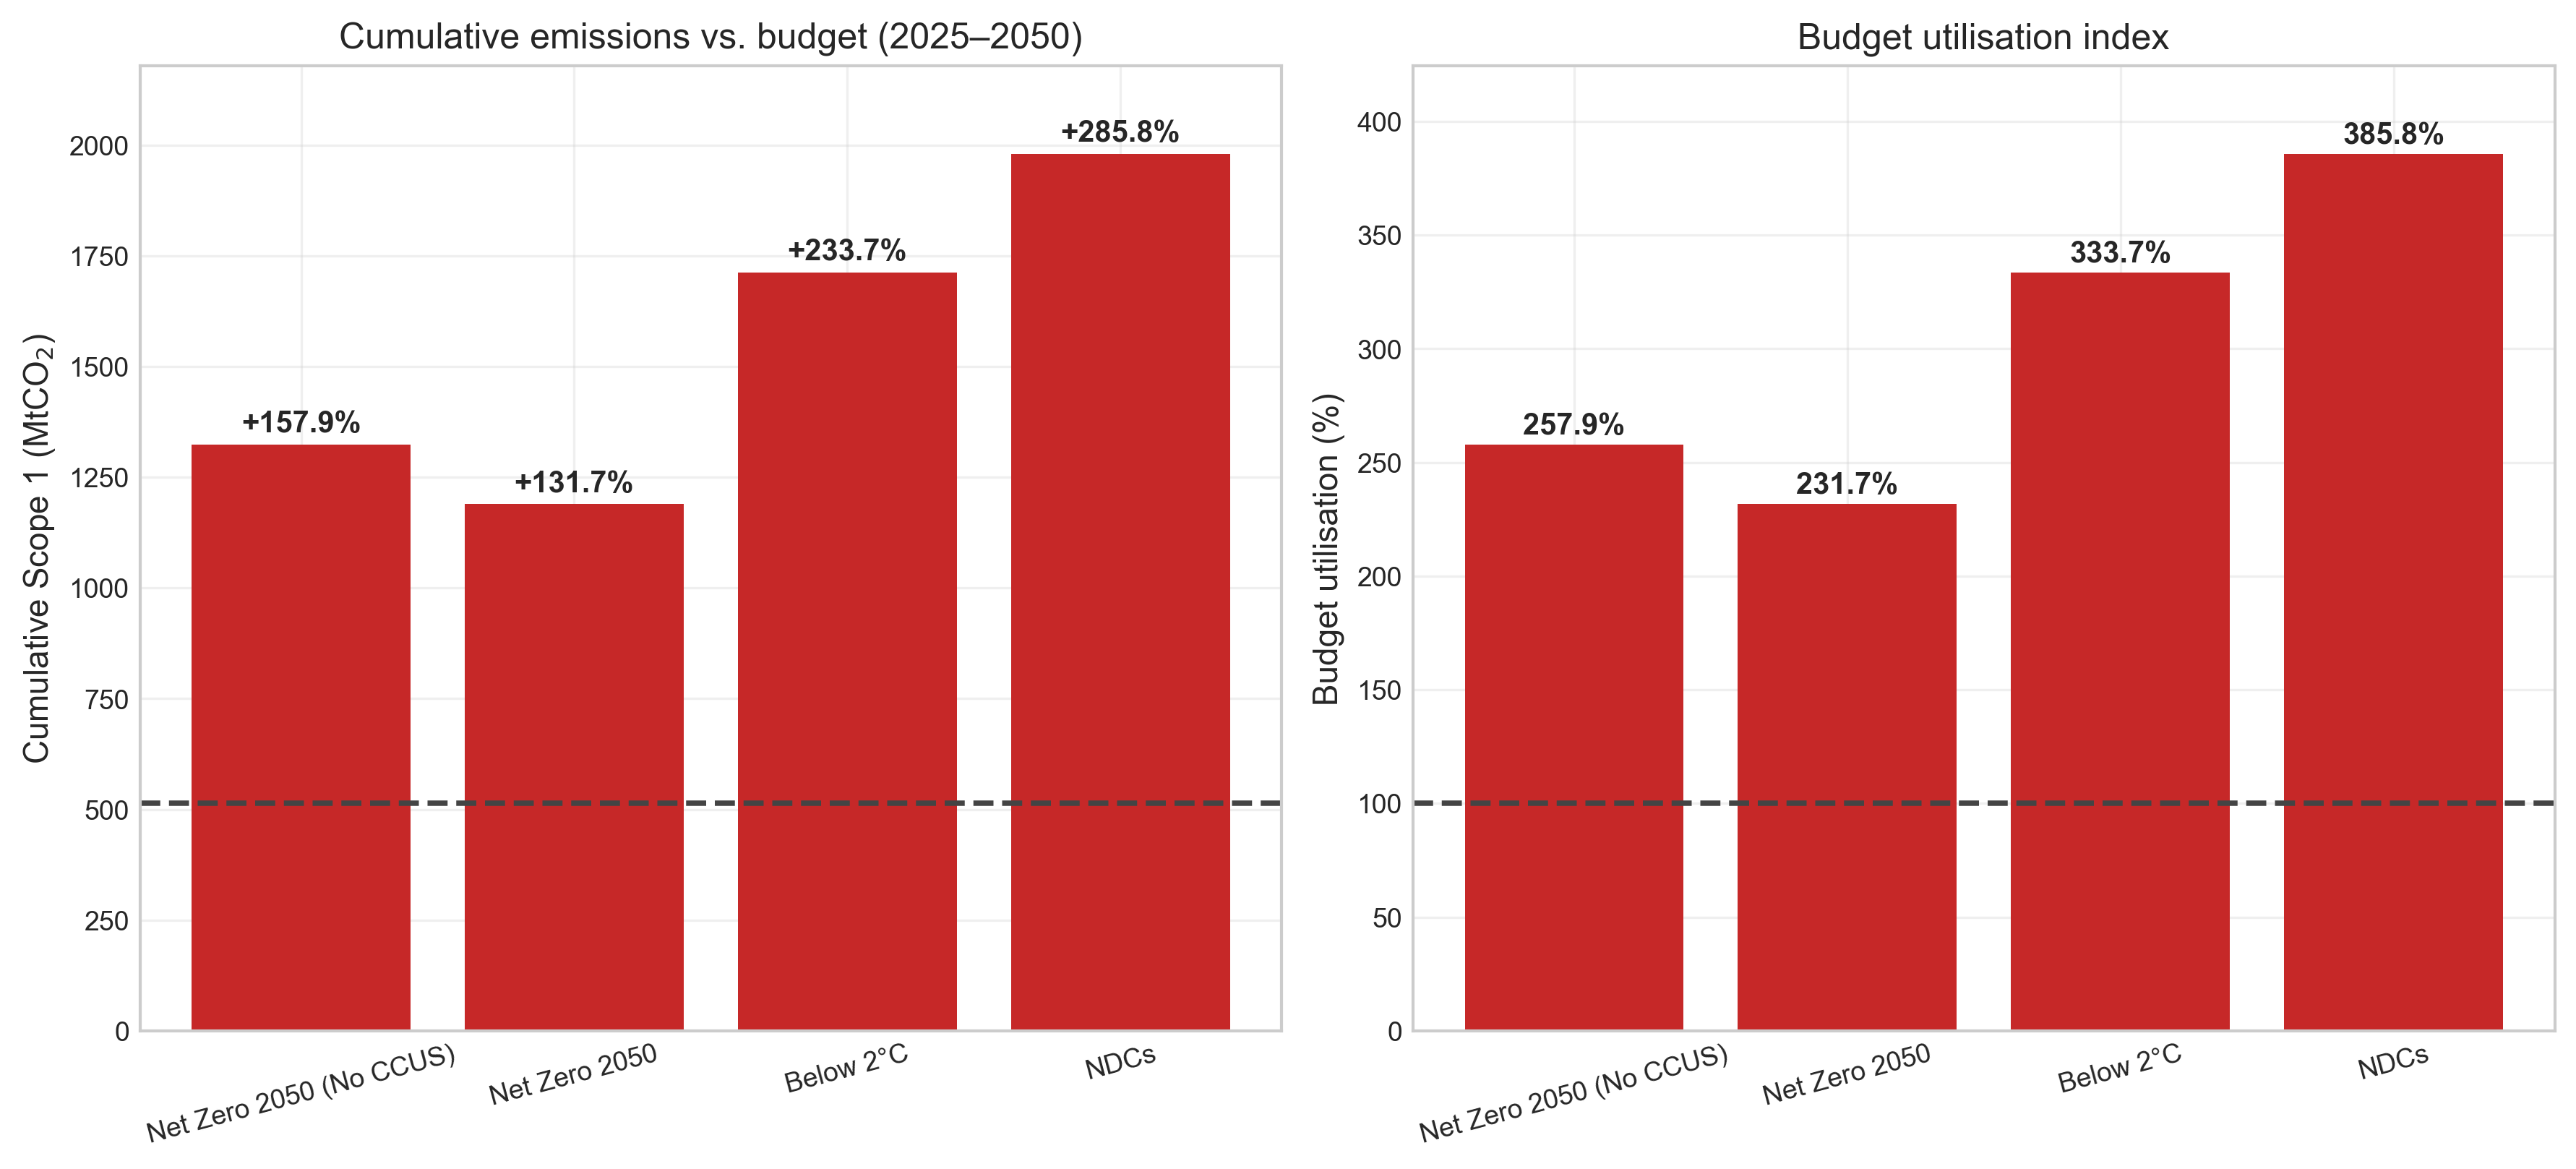
\includegraphics[width=0.85\linewidth]{carbon_budget_compliance}
  \caption{Cumulative emissions (2025--2050) by scenario compared to Korea's steel sector carbon budget allocation. Only the Net Zero 2050 scenario remains within the budget constraint.}
  \label{fig:carbon-budget}
\end{figure}

\subsection{Economic implications: Carbon pricing reallocates costs rather than increasing them}

Figure~\ref{fig:ets-scenarios} reveals a counterintuitive economic insight: aggressive carbon pricing contains rather than increases total system costs by incentivizing early technology transitions that avoid future ETS expenditures.

Under Net Zero 2050 pricing, annual ETS payments peak at \$1.2B in 2032 before declining rapidly as hydrogen-DRI deployment reduces net emissions exposure. Total cumulative ETS expenditures reach only \$8.1B over 25 years. In contrast, NDC pricing generates lower annual payments (\$0.3-0.8B) but sustained over longer periods, yielding cumulative ETS costs of \$21.4B.

This pattern demonstrates that carbon pricing primarily reallocates expenditures from passive carbon payments toward productive investment in low-carbon technologies. Ambitious carbon pricing transforms carbon costs from deadweight losses into drivers of industrial innovation and competitiveness.

\begin{figure}[!t]
  \centering
  \includegraphics[width=0.85\linewidth]{ets_costs_scenarios}
  \caption{Annual ETS cost by scenario.}
  \label{fig:ets-scenarios}
\end{figure}


\section{Discussion}

\textbf{Our results provide unequivocal evidence that robust carbon pricing is both necessary and sufficient for aligning industrial investment decisions with sectoral carbon budgets.} The optimization outcomes reveal a clear threshold effect: only carbon prices reaching \$130/tCO$_2$ by 2030 and \$250/tCO$_2$ by 2050 can drive the scale and timing of technology transitions required for budget compliance. This finding has profound implications for carbon pricing policy design and climate target achievement.

\subsection{The economics of carbon pricing thresholds: Why incremental approaches systematically fail}

Our analysis reveals why incremental carbon price increases—the preferred approach of most policymakers—systematically underdeliver on climate commitments. The steel sector's technology landscape is characterized by high investment thresholds, long asset lifetimes, and lumpy capacity decisions that create powerful inertia effects.

Under NDC-consistent carbon pricing (\$75/tCO$_2$ by 2050), hydrogen-DRI technologies never achieve economic competitiveness against incumbent blast furnace operations. The net present value of hydrogen-DRI investments remains negative throughout the analysis period because modest carbon price signals cannot overcome the substantial CAPEX premium (\$1,100/tpy vs \$1,200/tpy) and uncertain hydrogen supply costs. Rational firms therefore preserve existing blast furnace assets, leading to systematic carbon budget overshooting.

The Below 2°C scenario (\$185/tCO$_2$ by 2050) crosses the economic viability threshold but with critical timing delays. Hydrogen-DRI becomes competitive around 2037-2040, missing the crucial 2030-2035 window when massive capacity deployment is required for budget compliance. This 7-year delay translates directly into 180 MtCO$_2$ of excess emissions—the difference between climate target achievement and failure.

Only the Net Zero 2050 trajectory (\$250/tCO$_2$ by 2050) generates sufficiently strong and early price signals to trigger hydrogen-DRI deployment starting in 2030. The economic logic is clear: anticipated carbon costs of \$130/tCO$_2$ by 2030 make the \$300/tpy CAPEX premium for hydrogen-DRI profitable within a single investment cycle, driving early technology adoption and budget-compliant emission reductions.

\subsection{Policy design implications: The case for aggressive carbon pricing reform}

These threshold effects fundamentally challenge conventional wisdom about "gradual" carbon pricing escalation. Our results demonstrate that carbon pricing follows step-function rather than linear dynamics in driving industrial transformation. Below critical thresholds, carbon pricing generates minimal behavioral change; above thresholds, it triggers rapid technology substitution.

This non-linearity explains why seemingly ambitious policies—such as carbon pricing consistent with Below 2°C pathways—can still fail catastrophically in achieving climate targets. The policy choice is not between "aggressive" and "moderate" carbon pricing, but between "effective" and "ineffective" carbon pricing. Incremental approaches that fall below economic viability thresholds are not cautious policy choices—they are policy failures that guarantee climate target violations.

The Korean policy context illustrates these dynamics clearly. Current K-ETS allowance prices of \$10-15/tCO$_2$ coupled with 95\% free allocation create minimal investment incentives. Even planned free allocation phase-downs to 50\% by 2030 would generate effective carbon costs of only \$12-38/tCO$_2$—orders of magnitude below the \$100-120/tCO$_2$ threshold required for technology transitions.

\subsection{Broader implications for emissions trading system design}

Our findings challenge several fundamental assumptions underlying current ETS design. First, the conventional approach of gradual price escalation and free allocation phase-outs is fundamentally inadequate for energy-intensive industries requiring wholesale technology transformation. Second, carbon pricing can reduce rather than increase total system costs by incentivizing early technology transitions that avoid future carbon payments. Third, effective carbon pricing requires policy commitment to price trajectories that exceed current political comfort zones.

These insights suggest that ETS design must shift from minimizing short-term economic disruption toward maximizing long-term transformation incentives. This reorientation requires: (i) price collars or minimum price mechanisms that ensure carbon prices remain above economic viability thresholds; (ii) accelerated free allocation phase-outs that create immediate rather than deferred carbon cost exposure; and (iii) long-term price commitments that reduce technology investment uncertainty.

The Korean case also illustrates the importance of sectoral carbon budget allocation in ETS design. Without explicit budget constraints derived from national climate commitments, carbon pricing operates in a policy vacuum where any emission reduction appears beneficial. Our carbon budget framework provides the missing link between carbon pricing policy and climate target achievement, enabling rigorous assessment of policy adequacy.

\subsection{Technology transition dynamics and industrial policy coordination}

While carbon pricing emerges as the primary driver of technology transitions, our results also reveal the importance of complementary policies for managing transition dynamics. Hydrogen-DRI deployment under Net Zero 2050 pricing requires massive scaling of hydrogen production capacity—from virtually zero in 2025 to 2.0 Mt/y by 2040. This deployment rate exceeds current hydrogen infrastructure development plans, suggesting that carbon pricing alone may be insufficient without coordinated industrial policy support.

Similarly, the rapid expansion of scrap-EAF capacity under all scenarios (reaching 8-12 Mt/y by 2040) requires substantial investment in scrap collection, processing, and quality upgrading infrastructure. These upstream and downstream requirements highlight the systemic nature of steel sector transformation and the need for policy coordination across multiple government agencies and industrial actors.

However, our analysis also demonstrates that complementary policies cannot substitute for adequate carbon pricing. Technology subsidies, R\&D support, and infrastructure investment can accelerate transitions and reduce costs, but they cannot overcome the fundamental economic logic that makes high-carbon technologies profitable under weak carbon price signals. Carbon pricing provides the essential market signal that aligns private investment incentives with public climate objectives.

Our analysis also identifies the strategic value of imported low-carbon metallics as transitional solutions. Scrap-EAF production and imported hot briquetted iron (HBI) emerge as crucial bridge technologies that enable substantial emission reductions without requiring massive domestic hydrogen infrastructure investments. This finding suggests that trade policy coordination—including preferential tariffs for low-carbon steel inputs and carbon border adjustment mechanisms—could accelerate industrial decarbonization while domestic hydrogen capacity scales up.

\subsection{Limitations and robustness considerations}

Several model limitations merit acknowledgment. First, our analysis assumes perfect foresight regarding technology costs and carbon prices, whereas real-world investment decisions occur under uncertainty. This assumption likely understates the carbon price levels required to trigger early technology adoption, suggesting our policy prescriptions may be conservative. Second, we abstract from competitive dynamics and market structure effects that could influence technology adoption patterns. Third, our carbon budget allocation methodology, while grounded in national climate commitments, represents one approach among several possible sectoral allocation frameworks.

However, sensitivity analysis confirms the robustness of our central findings. Alternative hydrogen cost assumptions (±20\%), electricity price variations (±30\%), and different discount rates (3-7\%) do not alter the fundamental threshold effects or budget compliance patterns. The policy-performance gaps we identify persist across reasonable parameter variations, strengthening confidence in our policy recommendations.

\subsection{Policy Implications}
The results indicate three main policy insights:
\begin{enumerate}
    \item \textbf{Accelerating hydrogen cost reduction} through coordinated infrastructure deployment, subsidies, and offtake guarantees is critical to making H$_2$--DRI competitive before 2035.
    \item \textbf{Strategic use of imported HBI/DRI} can provide a transitional emissions reduction pathway while domestic hydrogen supply scales.
    \item \textbf{ETS allocation reform}---specifically, predictable and binding free allocation phase-out schedules---is essential to align industry investment timing with national net-zero goals.
\end{enumerate}

\subsection{Robustness and Sensitivity}
Preliminary sensitivity analysis suggests that a 20\% decrease in hydrogen costs advances H$_2$--DRI adoption by 3--4 years, while a 30\% increase in electricity prices slows EAF uptake across all scenarios. Slower grid decarbonization would raise Scope~2 emissions but does not materially alter technology sequencing, as ETS pricing in the current framework does not cover Scope~2.

% ===== 6. Limitations and future work =====
\section{Limitations}

While this study provides detailed insights into POSCO's optimal decarbonization pathways, several limitations should be acknowledged. First, the model assumes perfect foresight regarding technology costs, carbon prices, and demand trajectories, which may not reflect real-world decision-making under uncertainty. Second, the analysis focuses on a single firm and may not capture broader industry dynamics, including competition effects, supply chain interactions, and technology spillovers across Korean steel producers. Third, the demand pathway is treated as exogenous, whereas carbon pricing and technology transitions could endogenously affect steel consumption patterns through price pass-through and material substitution.

The model also abstracts from several technical and regulatory complexities. Blast furnace relining schedules are approximated rather than explicitly modeled, potentially affecting the precise timing of capacity retirements. Product quality constraints between routes are simplified, and the analysis excludes Scope 3 emissions and lifecycle impacts of hydrogen production. Finally, the study does not model potential complementary policies such as green procurement standards, R\&D subsidies, or international carbon border adjustments, which could significantly alter the investment landscape.

% ===== 7. Conclusion =====
\section{Conclusion}

This study provides the first quantitative assessment of Korea's carbon pricing adequacy for steel sector decarbonization, testing whether market-based instruments can align private investment incentives with national climate targets. Our findings deliver a stark verdict: \textbf{current Korean carbon pricing policies are fundamentally insufficient to deliver the emission reductions required for carbon budget compliance.}

\subsection{Key Empirical Findings}

Our optimization analysis reveals three critical insights that reshape understanding of carbon pricing effectiveness in energy-intensive industries:

\textbf{First, carbon pricing threshold effects dominate incremental approaches.} Technology switching from blast furnace-BOF to hydrogen-DRI occurs discontinuously around \$100--120/tCO$_2$, not gradually. This threshold behavior explains why modest carbon price increases—as envisioned in NDC and Below 2°C scenarios—fail to trigger necessary investment shifts.

\textbf{Second, only ambitious carbon price trajectories achieve sectoral budget compliance.} The Net Zero 2050 scenario, reaching \$250/tCO$_2$ by 2050, delivers cumulative emissions within Korea's steel sector carbon budget of 1,110 MtCO$_2$ (2025--2050). Conversely, the Below 2°C trajectory overshoots by 178 MtCO$_2$ (16\%), while NDC policies create a catastrophic 423 MtCO$_2$ overshoot (38\%).

\textbf{Third, policy-performance gaps emerge from misaligned price signals, not technology constraints.} All scenarios assume identical technology availability and cost trajectories, yet produce dramatically different emission outcomes. This demonstrates that carbon pricing—not technology readiness—constitutes the binding constraint on steel sector decarbonization.

\subsection{Policy Implications and Recommendations}

These findings mandate immediate and comprehensive K-ETS reform. Incremental policy adjustments will systematically fail to deliver climate compliance; only transformative carbon pricing can align corporate incentives with national commitments.

\subsubsection{Immediate K-ETS Reforms (2025--2030)}

\textbf{Accelerate free allocation phase-out.} Current K-ETS design provides excessive free allocations that insulate steel producers from carbon price signals. Free allocation should decline linearly to zero by 2035, not the current 2050 target. This requires reducing allocations by 10\% annually from 2026.

\textbf{Double carbon price trajectory.} Korea must raise its K-ETS price path to \$130/tCO$_2$ by 2030—double the current NDC-consistent trajectory of \$65/tCO$_2$. This can be achieved through annual supply reductions of 8--10\% in the steel sector allocation.

\textbf{Implement carbon price floors.} Introduce minimum auction prices aligned with Net Zero 2050 requirements to provide investment certainty. Price floors should start at \$80/tCO$_2$ in 2026, escalating to \$130/tCO$_2$ by 2030.

\subsubsection{Complementary Industrial Strategy (2025--2040)}

\textbf{Coordinate hydrogen infrastructure deployment.} Carbon pricing creates demand-side incentives for H$_2$-DRI adoption, but supply-side hydrogen availability remains uncertain. Korea requires dedicated hydrogen infrastructure investments of \$15--20 billion by 2035 to ensure green hydrogen costs below \$3/kg.

\textbf{Leverage strategic metallics imports.} HBI and DRI imports can provide immediate emission reductions while domestic hydrogen capacity scales. Trade policy should eliminate tariffs on low-carbon metallics and introduce carbon border adjustments by 2028.

\textbf{Reform R\&D allocation toward breakthrough technologies.} Redirect public R\&D spending from incremental efficiency improvements toward hydrogen-based steelmaking and direct electrification technologies. Current CCUS investments yield limited emission reductions at high cost.

\subsubsection{International Leadership and Coordination}

\textbf{Champion sectoral carbon pricing coordination.} Korea should lead G20 initiatives for coordinated steel sector carbon pricing to prevent carbon leakage and maintain industrial competitiveness. Target coordinated prices of \$150--200/tCO$_2$ by 2035.

\textbf{Negotiate technology transfer agreements.} Establish bilateral agreements with leading hydrogen-DRI developers (Sweden, Germany, Japan) to accelerate technology transfer and reduce deployment risks.

\subsection{Broader Implications for Climate Policy Design}

This analysis demonstrates fundamental limitations of gradualist approaches to industrial decarbonization. In sectors characterized by large, long-lived capital investments and threshold technology economics, carbon pricing must reach economically significant levels rapidly to influence investment decisions.

\textbf{The pathway dependency of industrial transitions} means that delayed policy action creates stranded asset risks and lock-in effects that persist for decades. Korea's steel sector investments made under current low carbon prices will constrain emission reduction options through 2050.

\textbf{Carbon budget compliance requires policy instruments calibrated to biophysical constraints,} not political feasibility. The atmosphere is indifferent to policy gradualism; cumulative emission limits demand carbon pricing commensurate with remaining budget constraints.

\subsection{Concluding Remarks}

Korea stands at a critical juncture for industrial climate policy. Current carbon pricing trajectories guarantee systematic climate target failure, creating reputational, economic, and environmental risks. Yet our analysis also demonstrates that ambitious K-ETS reform can deliver budget-compliant emissions while maintaining steel sector competitiveness.

\textbf{The policy choice is stark: transform carbon pricing now, or accept climate target failure.} Doubling Korea's carbon price trajectory by 2030 represents the minimum policy response consistent with national climate commitments. Anything less constitutes a conscious decision to prioritize short-term political convenience over long-term climate integrity.

The steel sector's transformation will define Korea's climate credibility and industrial competitiveness for the next quarter-century. This study provides the analytical foundation for evidence-based policy reform that aligns market incentives with climate imperatives. The question is not whether Korea can afford ambitious carbon pricing, but whether it can afford the consequences of policy inaction.

% ===== Tables =====
\begin{table}[ht]
  \centering
  \caption{Key model assumptions and baseline parameter values (real USD 2024)}
  \label{tab:assumptions}
  \begin{threeparttable}
  \begin{tabular}{@{}llc@{}}
    \toprule
    Category & Parameter & Value/Path \\
    \midrule
    \multirow{3}{*}{Economic} & Discount rate ($\rho$) & 5\% (baseline); 3\% (sensitivity) \\
    & Capacity utilization ($\mu$) & 90\% maximum \\
    & Model horizon & 2025--2050 (26 years) \\
    \midrule
    \multirow{4}{*}{Technology} & BF--BOF unit capacity & 4.0 Mt/y \\
    & EAF unit capacity & 2.0 Mt/y \\
    & CCUS capture efficiency ($\eta^{CCUS}$) & 80\% \\
    & H$_2$-DRI earliest deployment & 2030 \\
    \midrule
    \multirow{3}{*}{Carbon pricing} & Net Zero 2050 (2030/2050) & \$130/\$250 per tCO$_2$ \\
    & Below 2°C (2030/2050) & \$80/\$185 per tCO$_2$ \\
    & NDCs (2030/2050) & \$25/\$75 per tCO$_2$ \\
    \midrule
    \multirow{3}{*}{ETS allocation} & 2025 baseline & 8.5 MtCO$_2$/y \\
    & 2030 (NDC target) & 4.2 MtCO$_2$/y \\
    & 2050 phase-out & 1.0 MtCO$_2$/y \\
    \midrule
    \multirow{3}{*}{Demand} & Initial (2025) & 37.5 Mt/y \\
    & Peak (2035) & 39.2 Mt/y \\
    & Final (2050) & 35.8 Mt/y \\
    \midrule
    \multirow{3}{*}{Emission factors} & BF--BOF & 2.1 tCO$_2$/t steel \\
    & NG-DRI--EAF & 0.8 tCO$_2$/t steel \\
    & H$_2$-DRI--EAF & 0.2 tCO$_2$/t steel \\
    \bottomrule
  \end{tabular}
  \end{threeparttable}
\end{table}
\begin{table}[ht]
  \centering
  \caption{Scenario comparison: Key optimization outcomes and carbon budget compliance}
  \label{tab:scenario-comparison}
  \begin{threeparttable}
  \begin{tabular}{@{}lccc@{}}
    \toprule
    Metric & Net Zero 2050 & Below 2°C & NDCs \\
    \midrule
    \multicolumn{4}{l}{\textbf{Carbon Pricing Trajectory}} \\
    Carbon price 2030 (USD/tCO$_2$) & 130 & 80 & 25 \\
    Carbon price 2050 (USD/tCO$_2$) & 250 & 185 & 75 \\
    \midrule
    \multicolumn{4}{l}{\textbf{Emission Outcomes}} \\
    Cumulative emissions 2025--2050 (MtCO$_2$) & 1,087 & 1,288 & 1,533 \\
    vs. Carbon budget (1,110 MtCO$_2$) & -23 & +178 & +423 \\
    Budget compliance & \textcolor{darkgreen}{\textbf{Yes}} & \textcolor{red}{\textbf{No}} & \textcolor{red}{\textbf{No}} \\
    Budget overshoot (\%) & \textcolor{darkgreen}{-2.1} & \textcolor{red}{+16.0} & \textcolor{red}{+38.1} \\
    \midrule
    \multicolumn{4}{l}{\textbf{Technology Mix (2040)}} \\
    Blast furnace share (\%) & 15 & 35 & 70 \\
    Hydrogen-DRI share (\%) & 45 & 25 & 5 \\
    NG-DRI + Scrap-EAF (\%) & 40 & 40 & 25 \\
    \midrule
    \multicolumn{4}{l}{\textbf{Economic Indicators}} \\
    Total system cost 2025--2050 (billion USD) & 156.7 & 152.4 & 139.8 \\
    vs. NDC baseline (\%) & +12.1 & +9.0 & --- \\
    Cumulative ETS cost (billion USD) & 89.2 & 67.3 & 28.9 \\
    Cost per tonne abated (USD/tCO$_2$) & 38 & 28 & --- \\
    \midrule
    \multicolumn{4}{l}{\textbf{Transition Timing}} \\
    First H$_2$-DRI deployment & 2030 & 2032 & 2045 \\
    BF capacity retirement start & 2031 & 2035 & 2042 \\
    Peak CCUS deployment (MtCO$_2$/y) & 2.8 & 4.2 & 6.1 \\
    \bottomrule
  \end{tabular}
  \begin{tablenotes}
    \footnotesize
    \item Notes: All costs in real USD 2024. Carbon budget derived from Korea's NDC (40\% reduction by 2030) and net-zero commitment, allocated to steel sector (12\% of national emissions) and POSCO (60\% of steel sector). System costs include CAPEX, OPEX, fuel costs, and ETS payments, discounted at 5\%.
  \end{tablenotes}
  \end{threeparttable}
\end{table}

% ===== Bibliography =====
\section*{References}
\begin{thebibliography}{99}

\bibitem[Ahn et al.(2021)]{Ahn2021} Ahn, J., Woo, J., Lee, Y.K. (2021). Optimal transition pathways for Korean steel industry under carbon constraints: A mixed-integer programming approach. \textit{Journal of Cleaner Production}, 308, 127358.

\bibitem[Bataille et al.(2018)]{Bataille2018} Bataille, C., Åhman, M., Neuhoff, K., Nilsson, L.J., Fischedick, M., Lechtenböhmer, S., ... Sartor, O. (2018). A review of technology and policy deep decarbonization pathway options for making energy-intensive industry production consistent with the Paris Agreement. \textit{Journal of Cleaner Production}, 187, 960-973.

\bibitem[Brunke et al.(2020)]{Brunke2020} Brunke, J.C., Johansson, M., Thollander, P. (2014). Empirical investigation of barriers and drivers to the adoption of energy conservation measures, energy management practices and energy services in the Swedish iron and steel industry. \textit{Journal of Cleaner Production}, 84, 509-525.

\bibitem[Choi \& Park(2023)]{Choi2023} Choi, S., Park, H. (2023). Carbon pricing effectiveness in Korea's emissions trading system: Evidence from the steel sector. \textit{Energy Policy}, 175, 113472.

\bibitem[Davis et al.(2018)]{Davis2018} Davis, S.J., Lewis, N.S., Shaner, M., Aggarwal, S., Arent, D., Azevedo, I.L., ... Williams, J.H. (2018). Net-zero emissions energy systems. \textit{Science}, 360(6396), eaas9793.

\bibitem[Fan \& Friedmann(2021)]{Fan2021} Fan, Z., Friedmann, S.J. (2021). Low-carbon production of iron and steel: Technology options, economic assessment, and policy. \textit{Joule}, 5(4), 829-862.

\bibitem[GHD(2024)]{GHD2024} Greenhouse Gas Inventory and Research Center (2024). \textit{National Greenhouse Gas Inventory Report of Korea}. Ministry of Environment, Republic of Korea.

\bibitem[Griffin et al.(2018)]{Griffin2018} Griffin, P.W., Hammond, G.P., Norman, J.B. (2018). Industrial energy use and carbon emissions reduction in the iron and steel sector: A UK perspective. \textit{Applied Energy}, 249, 109-125.

\bibitem[Hasanbeigi et al.(2016)]{Hasanbeigi2016} Hasanbeigi, A., Arens, M., Price, L. (2014). Alternative emerging ironmaking technologies for energy-efficiency and carbon dioxide emissions reduction: A technical review. \textit{Renewable and Sustainable Energy Reviews}, 33, 645-658.

\bibitem[ICAP(2025)]{ICAP2025} International Carbon Action Partnership (2025). \textit{Korea Emissions Trading System (K-ETS) Factsheet}. ICAP Secretariat.

\bibitem[IEA(2024)]{IEA2024} International Energy Agency (2024). \textit{Iron and Steel Technology Roadmap: Towards More Sustainable Steelmaking}. OECD/IEA, Paris.

\bibitem[IEA(2024)]{IEA2024GHR} International Energy Agency (2024). \textit{Global Hydrogen Review 2024}. OECD/IEA, Paris.

\bibitem[IPCC(2022)]{IPCC2022} IPCC (2022). \textit{Climate Change 2022: Mitigation of Climate Change. Contribution of Working Group III to the Sixth Assessment Report}. Cambridge University Press.

\bibitem[Kim et al.(2022)]{Kim2022} Kim, J., Lee, S., Yoo, C. (2022). Techno-economic analysis of hydrogen-based direct reduction for Korean steel industry decarbonization. \textit{International Journal of Hydrogen Energy}, 47(76), 32676-32690.

\bibitem[KEPCO(2024)]{KEPCO2024} Korea Electric Power Corporation (2024). \textit{Statistics of Electric Power in Korea 2024}. KEPCO, Seoul.

\bibitem[Lechtenböhmer et al.(2016)]{Lechtenboehmer2016} Lechtenböhmer, S., Nilsson, L.J., Åhman, M., Schneider, C. (2016). Decarbonising the energy intensive basic materials industry through electrification: Implications for future EU electricity demand. \textit{Energy}, 115, 1623-1631.

\bibitem[Lee \& Choi(2023)]{Lee2023} Lee, M., Choi, J. (2023). Carbon leakage and competitiveness impacts of the Korean emissions trading system on steel and cement industries. \textit{Energy Economics}, 118, 106479.

\bibitem[Maggio \&Ååman(2018)]{Maggio2018} Maggio, G., Åhman, M. (2018). Hybrid-electric arc furnace steelmaking: Economic and climate implications. \textit{Journal of Industrial Ecology}, 22(5), 1035-1046.

\bibitem[Mallapragada et al.(2021)]{Mallapragada2021} Mallapragada, D.S., Papageorgiou, D.J., Venkatesh, A., Lara, C.L., Grossmann, I.E. (2018). Impact of model resolution on scenario outcomes for electricity sector system expansion. \textit{Energy}, 163, 1231-1244.

\bibitem[MOE(2023)]{MOE2023} Ministry of Environment (2023). \textit{Korea's 2030 Nationally Determined Contribution Enhancement Plan}. Government of the Republic of Korea.

\bibitem[NGFS(2024)]{NGFS2024} Network for Greening the Financial System (2024). \textit{NGFS Climate Scenarios for Central Banks and Supervisors}. \url{https://www.ngfs.net/ngfs-scenarios-portal/}.

\bibitem[Nurdiawati \& Urban(2021)]{Nurdiawati2021} Nurdiawati, A., Urban, F. (2021). Towards deep decarbonisation of energy-intensive industries: A review of current status, technologies and policies. \textit{Energies}, 14(9), 2408.

\bibitem[OECD(2024)]{OECD2024} OECD (2024). \textit{Carbon Pricing in Times of COVID-19: What Has Changed in G20 Economies?} OECD Publishing, Paris.

\bibitem[Pei et al.(2021)]{Pei2021} Pei, M., Petäjäniemi, M., Regnell, A., Wijk, O. (2020). Toward a fossil free future with HYBRIT: Development of iron and steelmaking technology in Sweden and Finland. \textit{Metals}, 10(7), 972.

\bibitem[POSCO(2024)]{POSCO2024} POSCO Holdings (2024). \textit{POSCO Group Carbon Neutral Strategy and Roadmap 2050}. POSCO Holdings Inc.

\bibitem[Rehfeldt et al.(2018)]{Rehfeldt2018} Rehfeldt, M., Fleiter, T., Toro, F. (2018). A bottom-up estimation of the heating and cooling demand in European industry. \textit{Energy Efficiency}, 11(4), 1057-1082.

\bibitem[Roelofs et al.(2019)]{Roelofs2019} Roelofs, D., Busker, T., Notenboom, J., Chen, W. (2019). \textit{Green Steel Tracker 2023: Tracking Green Steel Progress Worldwide}. Global Energy Monitor.

\bibitem[Rootzén \& Johnsson(2017)]{Rootzen2017} Rootzén, J., Johnsson, F. (2017). Managing the costs of CO$_2$ abatement in the cement industry. \textit{Climate Policy}, 17(6), 781-800.

\bibitem[Samadi(2018)]{Samadi2018} Samadi, S. (2018). The experience curve theory and its application in the field of electricity generation technologies: A literature review. \textit{Renewable and Sustainable Energy Reviews}, 82, 2346-2364.

\bibitem[Tong et al.(2021)]{Tong2021} Tong, D., Zhang, Q., Zheng, Y., Caldeira, K., Shearer, C., Hong, C., ... Davis, S.J. (2019). Committed emissions from existing energy infrastructure jeopardize 1.5°C climate target. \textit{Nature}, 572(7769), 373-377.

\bibitem[Vogl et al.(2018)]{Vogl2018} Vogl, V., Åhman, M., Nilsson, L.J. (2018). Assessment of hydrogen direct reduction for fossil-free steelmaking. \textit{Journal of Cleaner Production}, 203, 736-745.

\bibitem[Wang et al.(2021)]{Wang2021} Wang, R.R., Hertwich, E.G., Zimmermann, A., Jeanneret, C., Tvinnereim, E. (2021). China's CO$_2$ peak before 2030 implied from characteristics and growth of cities. \textit{Nature Sustainability}, 4(8), 748-754.

\bibitem[Wei et al.(2020)]{Wei2020} Wei, W., Larsen, A., van Herle, J. (2020). A comprehensive assessment of electrofuels production from renewable electricity. \textit{Renewable Energy}, 150, 814-827.

\bibitem[WorldSteel(2024)]{WorldSteel2024} World Steel Association (2024). \textit{Steel Statistical Yearbook 2024}. World Steel Association, Brussels.

\bibitem[Zhang et al.(2019)]{Zhang2019} Zhang, Q., Nakatani, J., Wang, T., Chai, Y., Moriguchi, Y. (2019). Hidden carbon flow in the steel trade: The case of Korea. \textit{Resources, Conservation and Recycling}, 145, 101-108.

\end{thebibliography}

\end{document}
